
%%%% contact via <kisfg@hotmail.com, haikureimu@hnu.edu.cn>
% tikzcd 和 dvipdfmx 冲突的处理方法:https://fohte.hateblo.jp/entry/2017/02/03/130829
% 在documentclass处提供dvipdfmx的选项。
% 必须要包含,否则无法插入 png。
\documentclass[12pt, a4paper]{article}

% 需要传入dvipfmx 参数使插图正常工作。
\usepackage[
    dvipdfmx            % 必要项,支持最终dvipdfmx对tikzcd插图处理
] {graphicx}             
\usepackage{subcaption}
\usepackage{caption}
\usepackage[
    figuresright
] {rotating}            % 用于旋转某些东西,如长表格。
\usepackage[
    includeheadfoot
] {geometry}            % 调节页边距。
\usepackage{tikz-cd}
\usepackage{tikz}
% 左边距 3cm
% 右边距 2cm
% left=3cm,
% right=2cm,
\geometry{
    left=3cm,
    right=2cm
}
\usepackage{enumerate}  % 罗列编号用的宏包
\usepackage{titlesec}   % 控制标题的宏包
\usepackage{titletoc}   % 控制目录的宏包
\usepackage{fancyhdr}   % fancyhdr宏包 支持页眉和页脚的相关定义
\usepackage[UTF8]{ctex} % 支持中文显示
\usepackage{color}      % 支持彩色
\usepackage[
    scr=boondox,
    cal=esstix
] {mathalpha}           % mathcal 正确显示
\usepackage{
    amsmath, 
    amsthm, 
    amssymb, 
    amsbsy,
    % txfonts,          % 课本里头用的公式字体类型
    % mathptmx,         % 和 txfonts 是一家的
    % mathrsfs          % 书法字体包,有额外警报
    amsfonts,
}                       % 数学宏包
\usepackage[
    below               % 允许上一个section的浮动图形出现在下一个section的开始部分,还提供\FloatBarrier命令,使所有未处理的浮动图形立即被处理
] {placeins}                
\usepackage{flafter}    % 使得所有浮动体不能被放置在其浮动环境之前,以免浮动体在引述它的文本之前出现.
\usepackage{multirow}   % 使用Multirow宏包,使得表格可以合并多个row格
\usepackage{booktabs}   % 表格,横的粗线;\specialrule{1pt}{0pt}{0pt}
\usepackage{longtable}  % 支持跨页的表格。
\usepackage{tabularx}   % 自动设置表格的列宽
\usepackage{setspace}
\usepackage{float}      % 浮动体控制
\usepackage{balance}    % 自动调整超出margin的文字
\usepackage{enumitem}   % 使用enumitem宏包,改变列表项的格式
\usepackage{calc}       % 长度可以用+ - * / 进行计算

% \usepackage[
%     amsmath, 
%     thmmarks, 
%     hyperref
% ] {ntheorem}            
% 定理类环境宏包,其中 amsmath 选项用来兼容 AMS LaTeX 的宏包
\usepackage{indentfirst}% 首行缩进宏包
\usepackage{CJKutf8}    % 用在UTF8编码环境下,它可以自动调用CJK,同时针对UTF8编码作了设置。
\usepackage{CJK}
\usepackage{fancyhdr}   % 页眉页脚
\usepackage{lastpage}
\usepackage{layout}
\usepackage{overpic}
\usepackage[
    titles              % 保证目录换行
] {tocloft}
\usepackage{times}
\usepackage[
    backend=biber,      % 这个处理后端才能显示文献类型符如 [OL]
    style=gb7714-2015, 
    gbnamefmt=lowercase,% 外国人名小写 
    gbpub=false,
    gbalign=gb7714-2015,% 良好的左对齐
    gbnoauthor=true,    % 佚名作者用
    gbtype=true,        % 显式说明使用文献类型。
    gbpunctin=false
] {biblatex}

\usepackage[
    dvipdfm,
    unicode,
    pdfstartview=FitH,
    bookmarksnumbered=true,
    bookmarksopen=true,
    colorlinks=true,
    pdfborder={0 0 1},
    % 全部放黑。
    citecolor=black,
    linkcolor=black,
    anchorcolor=black,
    urlcolor=black,
    % breaklinks=true
] {hyperref}
\usepackage{ifthen}     % 条件编译可能会用得到
\usepackage[normalem]{ulem}
\useunder{\uline}{\ul}{}
%%%% contact via <kisfg@hotmail.com, haikureimu@hnu.edu.cn>
%%% 页边距定义
% 上边距 3cm
% 下边距 2.5cm
% 页眉到上边缘的距离 1.5cm
% 页脚到下边缘的距离 1.75cm
\setlength{\voffset}{0cm}
\setlength{\topmargin}{1.5cm-1in}
\setlength{\headheight}{13pt} % 页眉可以放得大一点
\setlength{\headsep}{1.5cm-12pt}
\setlength{\textheight}{\paperheight-5.5cm}
\setlength{\footskip}{0.75cm}

%%% 控制行距
\renewcommand{\baselinestretch}{1.5}
\setlength{\parindent}{2em}

%%% 定义字体
\newcommand{\song}{\songti}     % 宋体 rm
\newcommand{\hei}{\heiti}       % 黑体 bf 
\newcommand{\fs}{\fangsong}     % 仿宋体 tt
\newcommand{\kai}{\kaishu}      % 楷体 it
\newcommand{\li}{\lishu}        % 隶书
% 声明一个字体系列
% 使用新定义的字体系列
\renewcommand{\%}{\boldmath{\textsf{\char`\%}}}

%%%% 字号换算规范
%%%% 中文常用字号来代替国际用点数/磅/英寸/pt。
%% 参考 https://www.runoob.com/w3cnote/px-pt-em-convert-table.html
\newcommand{\chuhao}{\fontsize{42pt}{42pt}\selectfont}      % 初号, 1.倍行距
\newcommand{\yihao}{\fontsize{26pt}{26pt}\selectfont}       % 一号, 1.倍行距
\newcommand{\xiaoyi}{\fontsize{24pt}{24pt}\selectfont}      % 小一, 1.倍行距
\newcommand{\erhao}{\fontsize{22pt}{22pt}\selectfont}       % 二号, 1.倍行距
\newcommand{\xiaoer}{\fontsize{18pt}{18pt}\selectfont}      % 小二, 单倍行距
\newcommand{\sanhao}{\fontsize{16pt}{16pt}\selectfont}      % 三号, 1.倍行距
\newcommand{\xiaosan}{\fontsize{15pt}{15pt}\selectfont}     % 小三, 1.倍行距
\newcommand{\sihao}{\fontsize{14pt}{14pt}\selectfont}       % 四号, 1.0倍行距
\newcommand{\xiaosi}{\fontsize{12pt}{12pt}\selectfont}      % 小四, 1.倍行距
\newcommand{\wuhao}{\fontsize{10pt}{10pt}\selectfont}       % 五号, 单倍行距
\newcommand{\xiaowu}{\fontsize{8pt}{8pt}\selectfont}        % 小五, 单倍行距
\CJKtilde

\setitemize{leftmargin=3em,itemsep=0em,partopsep=0em,parsep=0em,topsep=-0em}
\setenumerate{leftmargin=3em,itemsep=0em,partopsep=0em,parsep=0em,topsep=0em}
\makeatletter
    \renewcommand\normalsize{
        \@setfontsize\normalsize{12pt}{12pt}
        \setlength\abovedisplayskip{4pt}
        \setlength\abovedisplayshortskip{4pt}
        \setlength\belowdisplayskip{\abovedisplayskip}
        \setlength\belowdisplayshortskip{\abovedisplayshortskip}
        \let\@listi\@listI}
    \def\defaultfont{\renewcommand{\baselinestretch}{2}\normalsize\selectfont}
    \setlength{\baselineskip}{20pt}
    \renewcommand{\CJKglue}{\hskip 0.5pt plus \baselineskip}
\makeatother

%% 这个块不要动,否则会引起 hyperref 的跳转错误。
\def\functor{\relax}
\let\functor\addcontentsline
\gdef\addcontentsline{\phantomsection\functor} % 这样就能修改addcontentsline的功能,使其额外插入。

%%% 配置目录
\renewcommand*{\contentsname}{\hfill 目\qquad\quad录 \hfill}
\setcounter{secnumdepth}{3}     % 编号深度 3
\setcounter{tocdepth}{3}        % 目录项深度为 3
\renewcommand{\thefigure}{\arabic{figure}}
\renewcommand{\thetable}{\arabic{table}}
\renewcommand{\theequation}{\arabic{equation}} % bold equation numbers
%% 目录项中的基本配件。
\renewcommand{\cftdot}{$...$}   % 点的样式。
\renewcommand{\cftdotsep}{1.5}  % TODO: 这里的单位是什么?

% 调整索引与文献名称之间的水平间距
\renewcommand{\biblabelsep}{6pt}

% section 从 1 开始计数
\renewcommand{\thesection}{\arabic{section}}
% section 格式配置
\titlecontents{section}[0em]    % 标题级别 标题位置 (左间距,理解为缩进)
    {\xiaosi\hei\vspace{0.5em}} % 标题样式
    {\textbf{\thecontentslabel}\hspace{0.5em}} 
    {} % 标题格式 (设置标题的整体格式,如字体尺寸、粗细、与上一个标题的垂直距离等,可空置)
    {\titlerule*[10pt]{\cftdot}\xiaosi\contentspage} 
    % 指引线与页码 (设置标题与页码之间的指引线样式以及页码的格式,该参数如果空置,标题将无指引线和页码)

% subsection 格式配置
\titlecontents{subsection}[2em]
    {\xiaosi\song\vspace{0.5em}}
    {\thecontentslabel\hspace{0.5em}}
    {}
    {\titlerule*[10pt]{\cftdot}\xiaosi\contentspage}

% subsubsection 格式配置
\titlecontents{subsubsection}[4em]
    {\xiaosi\song\vspace{0.5em}}
    {\thecontentslabel\hspace{0.5em}}
    {}
    {\titlerule*[10pt]{\cftdot}\xiaosi\contentspage}

%%% 图表目录以及格式定义。
\renewcommand*{\listfigurename}{\hfill 插图索引 \hfill}
\renewcommand*{\listtablename}{\hfill 附表索引 \hfill}
\setcounter{lofdepth}{1}
% figure index 的格式配置
\titlecontents{figure}[0em]
    {\xiaosi\song\vspace{0.5em}} %
    {图\hspace{0.5em}\textnormal{\thecontentslabel}\hspace{0.5em}}{} %
    {\titlerule*[10pt]{\cftdot}\xiaosi\contentspage}

% table index 的格式配置
\titlecontents{table}[0em]
    {\xiaosi\song\vspace{0.5em}} %
    {表\hspace{0.5em}\textnormal{\thecontentslabel}\hspace{0.5em}}{} %
    {\titlerule*[10pt]{\cftdot}\xiaosi\contentspage}

%% 设置插图目录条目的字体格式
% 直接重定义字体即可。
% https://tex.stackexchange.com/a/372825
% https://tex.stackexchange.com/a/192450
\DeclareCaptionFont{chineseBoldSongti}{\bfseries\songti\wuhao}
\DeclareCaptionFont{chineseWuHaoSongti}{\songti\wuhao}
\DeclareCaptionFont{chinesexiaowuSongti}{\songti\xiaowu}
\DeclareCaptionFont{chineseBoldHeiti}{\bfseries\heiti\wuhao}
\DeclareCaptionFont{chineseWuhao}{\wuhao}
\DeclareCaptionLabelFormat{figLabel}{#1~#2\hspace{0.5em}}
\captionsetup[figure]{
    name={\textbf{\song\wuhao{图}}},
    labelsep=space, % 去掉冒号
    labelformat=figLabel,
    font={chineseWuhao},          
    labelfont={bf},         
    textfont={chineseBoldSongti},   
    skip=0.5em,
}
\captionsetup[subfigure]{
    font={chineseWuhao},
    labelfont={chineseWuHaoSongti},
    textfont={chineseWuHaoSongti}
}
\DeclareCaptionLabelFormat{tabLabel}{#1~#2~}
\captionsetup[table]{
    name={\textbf{\hei\wuhao{表}}},
    labelsep=space, % 去掉冒号
    labelformat=tabLabel,
    font={chineseWuhao},
    labelfont={bf},         
    textfont={chineseBoldHeiti}, 
    skip=0.5em,       
}
%% 正文前罗马字体编号
\newcommand{\frontmatter}{
    \pagenumbering{Roman}
} 
\newcommand{\mainmatter} {%
    \clearpage{\cleardoublepage}
    \pagenumbering{arabic}
}

%%% 配置主目录中显示的节。
% 节
\titleformat{\section}{\sanhao\hei}{\thesection}{1em}{}
\titlespacing{\section}{0pt}{0pt}{12pt}
% 子节
\titleformat{\subsection}{\xiaosi\hei}{\thesubsection}{0.5em}{}
\titlespacing{\subsection}{0pt}{6pt}{6pt}
% 孙子节
\titleformat{\subsubsection}{\xiaosi\hei}{\thesubsubsection}{0.5em}{}
\titlespacing{\subsubsection}{0pt}{6pt}{6pt}

\renewcommand{\headrulewidth}{0pt}




%%% 制作前几页
%%% 定义特有字段以及特殊的变量和命令
\makeatletter
    %%% 封面配置
    % 校徽上的本科毕业论文(设计)
    \def\LieOnBadge#1{\def\@LieOnBadge{#1}}\def\@LieOnBadge{}
    % 封面页标题栏的第一行
    \def\titleOnTheFirstLine#1{\def\@titleOnTheFirstLine{#1}}\def\@titleOnTheFirstLine{}
    % 封面页标题栏的第二行
    \def\titleOnTheSecondLine#1{\def\@titleOnTheSecondLine{#1}}\def\@titleOnTheSecondLine{}
    % 中文标题,用于摘要页
    % 封面页标题栏的第一行
    \def\titleOnTheFirstLine#1{\def\@titleOnTheFirstLine{\xiaoer\hei{#1}}}\def\@titleOnTheFirstLine{}
    % 封面页标题栏的第二行
    \def\titleOnTheSecondLine#1{\def\@titleOnTheSecondLine{\xiaoer\hei{#1}}}\def\@titleOnTheSecondLine{}
    % 中文标题,用于摘要页
    \def\title#1{\def\@title{#1}}\def\@title{}
    % 英文标题,用于英文摘要页
    % 英文标题,用于英文摘要页
    \def\etitle#1{\def\@etitle{#1}}\def\@etitle{}
    % 文章作者
    \def\author#1{\def\@author{\centerline{\xiaosi\song{#1}}}}\def\@author{} 
    % 学号
    \def\studentid#1{\def\@studentid{\centerline{\xiaosi\song{#1}}}}\def\@studentid{}
    % 专业
    \def\subject#1{\def\@subject{\centerline{\xiaosi\song{#1}}}}\def\@subject{}
    % 院系
    \def\faculty#1{\def\@faculty{\centerline{\xiaosi\song{#1}}}}\def\@faculty{}
    % 指导老师
    \def\teacher#1{\def\@teacher{\centerline{\xiaosi\song{#1}}}}\def\@teacher{}
    % 文章日期
    \def\date#1{\def\@date{#1}}\def\@date{}
    %%% 页眉配置
    % 页眉说明
    \def\heading#1{\def\@heading{#1}}\def\@heading{}
    %%% 摘要配置
    % 中文摘要
    \long\def\cabstract#1{\long\def\@cabstract{#1}}\long\def\@cabstract{}
    % 英文摘要
    \long\def\eabstract#1{\long\def\@eabstract{#1}}\long\def\@eabstract{}
    %%% 关键词配置
    % 中文关键词
    \def\ckeywords#1{\def\@ckeywords{#1}}\def\@ckeywords{}
    % 英文关键词
    \def\ekeywords#1{\def\@ekeywords{#1}}\def\@ekeywords{}

    % 必须存在此句。
    \newlength{\@title@width}
    
    \newcommand{\makeheaders} {
        \setlength{\tabcolsep}{0em} % 做之前紧凑
        %% 封面
        \begin{titlepage}
            \centering
            % 湖南大学 毛主席题字
            \begin{figure*}[htp]
                \centering
                
\includegraphics[width=0.5\textwidth]{figures/hnu}
            \end{figure*}
            % 高清校徽
            \vspace{-1em}
            \begin{overpic}{figures/HSVGPDF}
                \put(4,75){\yihao \textbf{\texttt{HUNAN UNIVERSITY}}}
                \put(-35,40){\song\chuhao{\@LieOnBadge}}
            \end{overpic}\par
            \begin{table}[H]
                \centering
                \begin{tabular}{rrc}
                    % multicolumn 必须是第一条指令,前面只能是字体而不掺杂任何的命令。
                    \multicolumn{2}{r}{\xiaoer\hei{论文(设计)题目:}}\rule{0pt}{1.05cm} & \underline{\parbox[c]{6cm}{\@titleOnTheFirstLine}} \\
                    &\multicolumn{1}{r}{}\rule{0pt}{1.05cm}      & \underline{\parbox[c]{6cm}{\@titleOnTheSecondLine}} \\
                    \rule{0pt}{1.05cm}&\xiaosi\hei{学~生~姓~名 :} & \underline{\parbox[c]{6cm}{\@author}} \\
                    \rule{0pt}{1.05cm}&\xiaosi\hei{学~生~学~号 :} & \underline{\parbox[c]{6cm}{\@studentid}} \\
                    \rule{0pt}{1.05cm}&\xiaosi\hei{专~业~班~级 :} & \underline{\parbox[c]{6cm}{\@subject}} \\
                    \rule{0pt}{1.05cm}&\xiaosi\hei{学~院~名~称 :} & \underline{\parbox[c]{6cm}{\@faculty}} \\
                    \rule{0pt}{1.05cm}&\xiaosi\hei{指~导~老~师 :} & \underline{\parbox[c]{6cm}{\@teacher}} \\
                \end{tabular}
            \end{table}\par
            \vspace{2em}
            \centering{\xiaosi\hei{\the\year{} 年 \the\month{} 月 \quad 日}}
        \end{titlepage}
        \clearpage
    
        %% 从此往后页眉的格式固定。
        \def\headrule { 
            \if @fancyplain
                \let\headrulewidth\plainheadrulewidth
            \fi
            \hrule\@height 1.0pt \@width\headwidth\vskip1pt % 上面线为1pt粗
            \hrule\@height 0.5pt \@width\headwidth          % 下面0.5pt粗
            \vskip-2\headrulewidth\vskip-1pt                % 两条线的距离1pt
            \vspace{7mm}                                    % 双线与下面正文之间的垂直间距
        }
        \pagestyle{fancy}
        \fancyhf{}                      % 清空所有fancy样式,方便使页眉左部和右部置空
        \chead{\song\xiaowu{\@heading}} % 页眉上的字体大小
        \cfoot{\song\wuhao{\thepage}}   % 页码大小

        %%% 插入目录之中
        %% 授权书
        \addcontentsline{toc}{section}{毕业论文(设计)原创性声明和毕业论文(设计)版权使用授权书} { 
            \centerline{\hei\xiaoer{湖\hspace{0.5em}南\hspace{0.5em}大\hspace{0.5em}学}}\par
            \begin{center} \hei\xiaoer{毕业论文(设计)原创性声明} \end{center}\par
            \song\defaultfont{
                本人郑重声明:所呈交的论文(设计)是本人在导师的指导下独立进行研究所取得的研究成果。
                除了文中特别加以标注引用的内容外,本论文(设计)不包含任何其他个人或集体已经发表或撰写的成果作品。
                对本文的研究做出重要贡献的个人和集体,均已在文中以明确方式标明。
                本人完全意识到本声明的法律后果由本人承担。
            }\par\vspace{10pt}
            \song\xiaosi{学生签名:\hspace{10.5em}日期: \the\year{} 年 \hspace{.5em} 月 \hspace{.5em} 日}
            \vspace{0.5cm}
            \begin{center}\hei\xiaoer{毕业论文(设计)版权使用授权书}\end{center}
            \par\vspace{10pt}
            \song\defaultfont{
                本毕业论文(设计)作者完全了解学校有关保留、使用论文(设计)的规定,
                同意学校保留并向国家有关部门或机构送交论文(设计)的复印件和电子版,
                允许论文(设计)被查阅和借阅。本人授权湖南大学可以将本论文(设计)的全部或部分内容编入有关数据库进行检索,
                可以采用影印、缩印或扫描等复制手段保存和汇编本论文(设计)。
            }\par
            \song\defaultfont{{本论文(设计)属于}}\par
            \vspace{-0.25em}\hspace{7.5em}1、保 密□,在\underline{\hspace{4em}}年解密后适用于本授权书。\par
            \vspace{-0.25em}\hspace{7.5em}2、不保密□。\par
            \vspace{-0.25em}\hspace{7.5em}(请在以上相应方框内打``$\surd$'')\par
            \vspace{1em}
            \song\xiaosi{学生签名:\hspace{10.5em}日期: \the\year{} 年 \hspace{.5em} 月 \hspace{.5em} 日}
            \par\vspace{0.25em}
            \song\xiaosi{导师签名:\hspace{10.5em}日期: \the\year{} 年 \hspace{.5em} 月 \hspace{.5em} 日}
        }
        \clearpage

        %% 中文摘要  
        \addcontentsline{toc}{section}{摘~~要} {
            \begin{center}
                \hei\xiaoer{\@title}
            \end{center}
            \vspace{-10pt}
            \begin{center}
                \hei\xiaoer\ 摘\qquad 要
            \end{center}\par
            \song\defaultfont\@cabstract
            \vspace{\baselineskip}
            \hangafter=1\hangindent=52.3pt
            \newline\noindent
            {\hei\sihao{关键词:} \hei\xiaosi\@ckeywords}
        }
        \clearpage
        
        %% 英文摘要
        \addcontentsline{toc}{section}{Abstract} {
            \begin{center}
                \xiaoer{\textbf{\@etitle}}
            \end{center}\par
            \vspace{-12pt}
            \begin{center}
                \xiaoer\textbf{Abstract}
            \end{center}\par
            \vspace{-6pt}
            \defaultfont{\@eabstract}
            \vspace{\baselineskip}
            \hangafter=1\hangindent=60pt
            \newline\noindent
            {\xiaosi\textbf{Key Words:} \@ekeywords}
        }
        \newpage
        %% 图表以及目录
        \setlength{\tabcolsep}{0.5em} % 做完上述部分后,表格默认每个格子 0.5em 宽
    }

    \fancyhf{} % 清空所有fancy样式,方便使页眉左部和右部置空
    \pagestyle{fancy}
    \fancypagestyle{plain}{
        \fancyhead[C]{\song\xiaowu \@heading}
        \fancyfoot[C]{\song\xiaowu \thepage}
    }
    
\makeatother


\heading{湖南大学本科生毕业论文(设计)}
\LieOnBadge{本科生毕业论文(设计)}
% 标题全称、分行标题(如果首行够长则可忽略第二个)、分行标题二。
\title{川菜和湘菜在辣度上的对比研究}
\titleOnTheFirstLine{川菜和湘菜在辣度上}
\titleOnTheSecondLine{的对比研究}
\etitle{A Research Conducted on the Spiciness between SiChuan Cusine and Hunan Cusine}
% 作者以及导师
\author{十三香}
\studentid{201212313231}
\major{食品工程}
\faculty{后勤保障部}
\teacher{王守义}

% 声明书和授权内容。
%% 概要与关键词
% 这里填入你自己的内容。
\cabstract{
    摘要是论文内容的简要陈述,是一篇具有独立性和完整性的短文。
    摘要应包括本论文的创造性成果及其理论与实际意义。
    摘要中不宜使用公式、图表,不标注引用文献编号。避免将摘要写成目录式的内容介绍。
% 一定要有空行隔开,否则可能会缩成一坨。
    比如上面是一段,下面是第二段。

}
\eabstract{
    An abstract is a brief summary of a research article, 
    thesis, review, conference proceeding or any in-depth analysis of 
    a particular subject and is often used to help the reader quickly 
    ascertain the paper's purpose. When used, an abstract always 
    appears at the beginning of a manuscript or typescript, 
    acting as the point-of-entry for any given academic paper or patent application. 
    Abstracting and indexing services for various academic disciplines are aimed at 
    compiling a body of literature for that particular subject.
% There must be a blank setting right here to avoid the messing up of line-skip.
    As you can see, this paragraph has the same style as the previous one.

}
\ckeywords{关键词1;~~关键词2;~~关键词3;~~关键词4}
\ekeywords{Key Word1;~~Key Word 2;~~Key Word 3;~~Key Word 4}
%% 概要与关键词结束
%% 如果有需求可以加下面两行以在附录生成缩略表
% \glssetwidest{ADC}
% \makeglossaries
\clearpage
\graphicspath{{figures/}}
\addbibresource[location=local]{refer_ref.bib}
\begin{document}
	%% linux 下不可用 CJK
    \frontmatter
    %%% 前几页必要内容
    \makethesisheaders
    %%% 插图索引 可选项
    % 如果图片存在,则渲染
    \iftotalfigures {
        \addcontentsline{toc}{section}{插图索引}
        \listoffigures
        \clearpage
    }\fi
    %%% 附表索引 可选项
    % 如果表格存在,则渲染
    \iftotaltables {
        \addcontentsline{toc}{section}{附表索引}
        \listoftables
        \clearpage
    }\fi
    %%% 正文
    \mainmatter
    \begin{sloppypar} % 防止文字出界而自动调整的环境。
        \setcounter{page}{1}
        %% TOFIX: output-directory 和 include 冲突,尚未找到解决方案。
        \section{绪论}
    % 问题 方法 结论
    % 宇宙的真理 别人的结论 我的结论
    % 拿别人的东西来证明自己的论点
    % 避免洗稿
    你好世界。
\subsection{动机}
    本文的动机在于。
\subsection{贡献}
    本文在优化机制上所做出的贡献是。
\subsection{文章结构}
    本文编排的结构组织如下:第 \ref{section:relatedWork} 章介绍 eBPF 和 wasm 等相关工作;
    第 \ref{section:optimizations} 章介绍本文在两者优化机制上所做的贡献;
    第 \ref{section:experiment} 章介绍本文构建实验的方式和测试结果;
    第 \ref{section:discussion} 章将给出本文的讨论;
    第 \ref{section:conclusion} 章总结全文。

        \section{相关工作}
\label{section:relatedWork}
	\subsection{高级编程语言}
		% https://github.com/openjdk/jdk/blob/master/src/hotspot/share/compiler/compileTask.cpp
		\subsubsection{Java字节码解释器}
		Java虚拟机(JVM)转译和执行由Scala,Java,Groovy和Kotlin等高级编程语言编译得到的Java字节码。
		且当前的JVM系统由不同的组织和公司所开发,如Oracle开发的HotSpot\cite{OracleHotspot},
		阿里巴巴开发的DragonWell\cite{DragonWell}和IBM开发的OpenJ9\cite{IBMOpenJ9}。

		因JVM功能性复杂且规模巨大\cite{sonoyamaPerformanceStudyKotlin2021},所以潜在的缺陷不可避免\cite{jiaDetectingJVMJIT2023}。
		Jia,et al.\cite{jiaDetectingJVMJIT2023}观察到HotSpot公开的缺陷报告在每年的总数上虽然下降,但其即时编译器部分出现的缺陷却显著增加,
		有的甚至可以引起JVM的崩溃\cite{JVMcrashReport}。

		Chaliasos,et al.\cite{chaliasosWelltypedProgramsCan2021}通过按照表 \ref{jvmBugTracker} 所示的缺陷追踪网站,
		从中收集并整理出 4153 个已被修复且由测试用例确保不会再重现的缺陷;其工作还随机挑选了320个缺陷,结合开发者讨论以及缺陷报告,
		总结形成了五类的缺陷以及其根因,结果如图 \ref{JVMbugsRootCause} 所示。

		\begin{table}[H]
			\centering
			\caption{JVM类型缺陷的收集结果\parencite{chaliasosWelltypedProgramsCan2021}}
			\resizebox{\linewidth}{40pt}{
				\begin{tabular}{cccccccc}
					\specialrule{1pt}{1pt}{1pt}
					语言 &缺陷追踪网站 &链接 &问题总数 &最早记录时间 &最近记录时间 &缺陷收集 &后-筛选量(post-filtering)\\
					\hline
					Java   &Jira  &\url{https://bugs.openjdk.java.net/rest/api/latest/search} 	&10872 	&2004-02-11 &2021-03-26 &1252 &873  \\
					Scala2 &GitHub  &\url{https://api.github.com/repos/scala/bug} 				&12315 	&2003-05-22 &2021-03-11 &1180 &1067  \\
					Scala3 &GitHub  &\url{https://api.github.com/repos/lampepfl/dotty} 			&4286 	&2014-02-01 &2021-03-21 &429  &366 \\
					Kotlin &YouTrack  &\url{https://youtrack.jetbrains.com/api/issues} 			&40998 	&2011-10-28 &2021-04-09 &2189 &1601 \\
					Groovy &Jira  &\url{https://issues.apache.org/jira/rest/api/2/search} 		&9710 	&2003-09-25 &2021-04-09 &300  &246 \\
					\specialrule{1pt}{1pt}{1pt}
				\end{tabular}
			}
			\label{jvmBugTracker}
		\end{table}
		\begin{figure}[H]
			\centering
			\pgfplotstableread{
					index	         aa ee  cc dd    bb
				类型相关错误           90 4  10  4     21
				语义分析有误           22 2  30  3     20
				解析异常              42 1  13  7     14
				错误控制与报告不当      0  0  0   7     15
				AST转换不当            5  1  0   0     9
			}\jvmBugData
			\begin{tikzpicture}
				\begin{axis}
					[
						xbar,
						xbar stacked,
						ytick=data,
						bar width=0.5cm,
						ytick style={draw=none},
						width=0.5\linewidth,
						xmin=0,
						bar shift=0pt,
						axis y line*= none, axis x line*= none,
						yticklabels from table={\jvmBugData}{index},
						legend pos=outer north east,
						legend style={column sep=8pt,},
						point meta=x,
					]
					\addlegendimage{empty legend}\addlegendentry{\xiaowu\bf{JVM症状}}
					\addplot+ table [x=aa, meta=index, y expr=\coordindex] {\jvmBugData};\addlegendentry{\xiaowu{非预期编译时错误}}
					\addplot+ table [x=ee, meta=index, y expr=\coordindex] {\jvmBugData};\addlegendentry{\xiaowu{内部编译错误}}
					\addplot+ table [x=cc, meta=index, y expr=\coordindex] {\jvmBugData};\addlegendentry{\xiaowu{非预期运行时的表现}}
					\addplot+ table [x=dd, meta=index, y expr=\coordindex] {\jvmBugData};\addlegendentry{\xiaowu{误报}}
					\addplot+[
						nodes near coords,
						every node near coord/.append style={
							xshift=24pt,
							black,
						},
					] table [x=bb, meta=index, y expr=\coordindex] {\jvmBugData};\addlegendentry{\xiaowu{编译性能问题}}
				\end{axis}
			\end{tikzpicture}
			\caption{JVM各症状的错误原因分布\parencite{chaliasosWelltypedProgramsCan2021}}
			\label{JVMbugsRootCause}
		\end{figure}

		其中,AST转换不当是指编译器没有产生和原始输入程序在逻辑上保持一致的转换程序,占JVM缺陷的4.69\%,会引发非预期的编译时错误和内部编译错误。
		错误控制与报告不当是指JVM解释器正确辨识出程序错误,但错误处理和报告机制没有产生预期的响应结果。错误控制与报告不当占JVM缺陷的6.88\%,
		此类缺陷都与崩溃和错误报告有关。
		
		解析异常则是既不能解析一个标识符(即变量名、方法名或类名),也不能正确地检索到先前解析过的标识名。解析异常也占24.06\%,由两项原因所致:
		\begin{itemize}
			\item [(1)] 解析算法执行错误,如\href{https://bugs.openjdk.java.net/browse/JDK-7042566}{JDK-7042566}是在相同函数名下选择参数更多的一个来执行,
						从而引发错误;
			\item [(2)] 编译器错误查询;
			\item [(3)] 作用域状态错误。
		\end{itemize}
		
		语义分析有误则指的是解释器对特定程序代码生成了错误的分析结果,占JVM缺陷的24.06\%,由两方面原因所致:
		\begin{itemize}
			\item [(1)] 没有验证检查语义,如问题\href{https://github.com/scala/bug/issues/5878}{Scala2-5878};
			\item [(2)] 不正确的分析机制,如问题\href{https://github.com/scala/scala3/pull/4487}{Scala3-4487}。 
		\end{itemize}

		最后的类型相关错误指的是在前端编译器中运用类型系统内定义的规则以及类型中定义的操作应用于输入的源文件之中,但因实现不当而导致的错误。
		这一部分的实现不当是造成非预期编译时错误的主要原因,且以40.31\%(129/320)的比例使之成为JVM最常见的缺陷。且细分类型相关错误则仍有三组:
		\begin{itemize}
			\item [(1)] 不正确的类型推断和类型变量代替,如缺陷报告所报告的\href{https://youtrack.jetbrains.com/issue/KT-10711}{KT-10711};
			\item [(2)] 不正确的类型(强制或非强制)转换,如缺陷报告所报告的\href{https://youtrack.jetbrains.com/issue/KT-9630}{KT-9630};
			\item [(3)] 不正确的类型比较和边界计算,如缺陷报告所报告的\href{https://bugs.openjdk.org/browse/JDK-8284879}{JDK-8039214}。
		\end{itemize}

		\subsubsection{JavaScript字节码解释器}
		JavaScript(JS)是被广泛使用的编程语言之一,其迅速的发展由超过200万个可重用的npm软件库生态所支撑\cite{bhuiyanSecBenchjsExecutableSecurity2023}。
		JS常作为客户端一侧的web应用使用,驱动了当今世界上超过90\%的web页面\cite{Staicu2018SYNODEUA}。
		这种广泛的应用使得保证JS的安全性至关重要\cite{eomFuzzingJavaScriptInterpreters2024}。

		JS通过自身的执行引擎解释执行且主流浏览器提供商均实现并管理着其编写的js引擎。Google浏览器使用V8引擎\cite{v8Engine},
		Mozilla的火狐浏览器使用SpiderMonkey引擎\cite{MozillaSpiderMonkey},苹果公司的Safari浏览器使用WebKit\cite{WebKit}中的JS引擎,
		微软公司开发的Edge使用ChakraCore引擎\cite{ChakraCore}。这些引擎是浏览器的核心\cite{limSOKAnalysisWeb2021},依次将JS源码转变为字节码和机器码。

		而Ziyuan Wang et al.\cite{JSEngineBugs}汇总分析了V8,SpiderMonkey和Chakra三个主流JS引擎截至2022年
		已有的19019篇缺陷(bugs)报告,16437次修正和805个测试用例以及随机挑选的540个缺陷的根因,发现:
		\begin{itemize}
			\item[(1)] Compiler和DOM是存在缺陷最多的部件,结果如表 \ref{JSBuggySrc} 和表 \ref{JSBuggyComponents} 所示;
			\item[(2)] 小型测试用例足以触发多数漏洞,如V8中70.79\%的触发漏洞测试用例代码行数小于10行;
			\item[(3)] JS引擎漏洞修复通常不复杂,多数仅需修改少量代码行和文件。如V8中76.86\%的漏洞修复涉及代码行数少于100行;
			\item[(4)] 对于修复缺陷的时间,V8中有80.33\%的缺陷在半年内修复;SpiderMonkey引擎中有91.9\%的缺陷是在半年内修复,且有4.33\%是需要超过一年的时间才能修复;
			\item[(5)] 规范语义缺陷是最常见的根因。除此之外,执行缺陷、特性以及函数调用缺陷均比其它类型的缺陷多。与V8和Chakra相比,SpiderMonkey有更多构建错误和更少内存错误。
		\end{itemize}

		研究为确保后续研究的可复现性,还将其成果分别以BSD,MPL,MIT许可证颁布公开于Github上
		\footnote{\url{https://github.com/njuptw/Empirical-Study-V8}.}
		\footnote{\url{https://github.com/njuptw/Empirical-Study-SpiderMonkey}.}
		\footnote{\url{https://github.com/njuptw/Empirical-Study-Chakra}.}。

		另外,基于JavaScript的Node.js在服务器端和桌面端也得到大量的应用\cite{nodejsAbuse}。
		因缺乏浏览器的安全沙箱机制,eval和exec注入API可能会引发严重的危害\cite{holtskogSecurityNodejsTheory2023},
		同时因开发者对分析工具接受度低且修复意愿不足,模块间还存在责任推诿问题\cite{Staicu2018SYNODEUA}。

		\begin{table}[H]
			\centering
			\caption{2022年JS引擎缺陷在源码文件中的分布\parencite{JSEngineBugs}}
			\wuhao\songti{
				\begin{tabular*}{\textwidth}{@{}@{\extracolsep{\fill}}llllll@{}}
					\specialrule{1pt}{1pt}{1pt}
					\multicolumn{2}{c}{V8} &\multicolumn{2}{c}{SpiderMonkey} &\multicolumn{2}{c}{Chakra}\\
					\hline
					源文件 &缺陷数量 &源码 &缺陷数量 &源码 &缺陷数量\\
					\hline
					src/compiler  		&10525 		&js 			&3209 		&lib/Runtime/Library 			&4629 \\
					src/wasm  			&5070  		&dom 			&3082 		&lib/Runtime/Language 			&1984 \\
					src/builtins  		&4726  		&browser 		&2129 		&lib/Runtime/Base 				&1170 \\
					src/heap  			&3630  		&toolkit 		&1956 		&lib/Common/Memory 				&1004 \\
					src/objects  		&3087  		&third\_party 	&1933 		&lib/Runtime/ByteCode 			&1001 \\
					src/runtime  		&2571  		&gfx 			&1807 		&lib/Runtime/Types 				&883 \\
					src/parsing  		&2147  		&devtools 		&1136 		&lib/wabt/src 					&676 \\
					src/interpreter 	&1779  		&taskcluster 	&1022 		&lib/Runtime/Debug 				&582 \\
					src/crankshaft  	&1178  		&layout 		&1013 		&lib/WasmReader 				&514 \\
					src/ast  			&1141  		&intl 			&962  		&lib/Jsrt 						&482 \\
					src/full-codegen	&1089  		&netwerk 		&926  		&lib/Backend/arm64 				&264 \\
					src/debug  			&1073  		&modules 		&910  		&lib/Common/DataStructures 		&242 \\
					src/js  			&1049  		&js/src/jit 	&898  		&lib/common 					&240 \\
					src/ic  			&1034  		&mobile 		&730  		&lib/Common/Core 				&238 \\
					src/snapshot  		&1029  		&security 		&699  		&lib/Runtime/PlatformAgnostic 	&219 \\
					src/objects.cc 		&951   		&widget 		&540  		&lib/Backend/Lower.cpp 			&211 \\
					src/regexp  		&911   		&dom/media 		&534  		&lib/Backend/amd64 				&187 \\
					src/arm64  			&872   		&dom/base 		&468  		&lib/Parser/Parse.cpp 			&184 \\
					src/ia32  			&839   		&dom/ipc 		&367  		&lib/Backend/arm 				&170 \\
					src/arm  			&811   		&docshell 		&364  		&lib/Common/ConfigFlagsList.h 	&168\\
					\specialrule{1pt}{1pt}{1pt}
				\end{tabular*}
			}
			\label{JSBuggySrc}
		\end{table}	

		另外,S. Park et al.\cite{parkEmpiricalStudyPrioritizing2019}围绕JS引擎的漏洞问题,实现了CRScope用于分类安全与非安全的缺陷,
		并评估了Exploitable和AddressSanitizer等工具和模型的性能。其工作所用的训练数据集从Google、Mozilla、Microsoft的Edge与IE浏览器以及GitHub库中收集。
		内容上包含165个触发安全缺陷的JS Poc以及174个触发非安全缺陷的PoC。同时,S. Park et al.还编译了与PoC对应的JS引擎,
		构成727个二进制文件以及766个实例,用于训练模型判断崩溃问题是否由安全缺陷所引发。
		其数据集公开\footnote{\url{https://github.com/WSP-LAB/CRScope}.}以支撑后续研究。
		
		其训练模型和测试模型的方式采用了四折时间序列交叉验证方式\cite{kFoldCrossVerification},
		将所有安全和非安全漏洞按其在目标二进制文件中的提交日期排序,而后按升序排列崩溃实例并均分成5个桶,以保证每个桶中的崩溃实例数量大致相同(约153个)。
		评估实验结果显示,S. Park et al.所实现的CRScope则在Chakra、V8 和SpiderMonkey的崩溃实例上以0.85、0.89和0.93的准确度,
		优于Exniffer的0.51和AddressSanitizer的0.63。
		
		\begin{table}[H]
			\centering
			\caption{2022年JS引擎中各组件缺陷分布情况\parencite{JSEngineBugs}}
			\specialrule{1pt}{1pt}{1pt}
			\wuhao{
				\begin{subtable}[t]{\textwidth}
					\caption{Google开发的V8}
					\begin{tabular*}{\textwidth}{@{}@{\extracolsep{\fill}}llll@{}}
						\hline
						\multicolumn{2}{c}{未修复缺陷(5191)} & \multicolumn{2}{c}{已修复缺陷(2827)} \\
						\hline
						组件名 & 数量 &组件名称 &数量\\
						\hline
						编译器 & 932 & 编译器 & 565 \\
						WebAssembly & 855 & JS语法 & 553 \\
						JS语法 & 831 & Webassembly & 518 \\
						运行时 & 648 & 运行时 & 317 \\
						基础架构 & 446 & 垃圾回收 & 232 \\
						垃圾回收 & 435 & 人类语言国际化 & 227 \\
						人类语言国际化 & 338 & 基础架构 & 182 \\
						API & 253 & API & 111 \\
						构建文件 & 170 & 正则匹配 & 82 \\
						正则匹配 & 166 & 解释器 & 65\\
					\end{tabular*}
					\hline
				\end{subtable}
				\begin{subtable}[t]{\textwidth}
					\caption{Mozilla开发的SpiderMonkey}
					\begin{tabular*}{\textwidth}{@{}@{\extracolsep{\fill}}llll@{}}
						\hline
						\multicolumn{2}{c}{未修复缺陷(4499)} & \multicolumn{2}{c}{已修复缺陷(3502)} \\
						\hline
						组件名 & 数量 &组件名称 &数量\\
						\hline
						DOM &519 &DOM &428  \\
						常规 &397 &常规 &330  \\
						JavaScript &294 &JavaScript &252  \\
						图形 &251 &图形 &211  \\
						自动化发布 &152 &自动化发布 &143  \\
						页面布局 &149 &Web平台测试 &138  \\
						Web平台测试 &144 &页面布局 &127  \\
						网络 &142 &网络 &101  \\
						音视频 1&14 &WebRTC &88  \\
						WebRTC &107 &音视频 &79 \\
					\end{tabular*}
					\specialrule{1pt}{1pt}{1pt}
				\end{subtable}
			}
			\label{JSBuggyComponents}
		\end{table}

		\subsubsection{Lua字节码解释器}
		Lua是一个基于栈虚拟机的解释型语言,支持动态类型\cite{ierusalimschyLua54Reference2020}。
		Lua被设计为嵌入式语言,主要用于扩展应用程序,而非独立开发程序。它高度依赖宿主程序提供的API,
		标准库函数的加载也需由宿主程序显式完成\cite{SecurityLuaSandbox2022}。
		Lua官方在其官网有单独开设一个页面用于记录其解释器存在的缺陷\footnote{\url{https://www.lua.org/bugs.html}.}。
		同时还提供了各个版本的手册\footnote{\url{https://www.lua.org/manual/}.}以方便编程人员查阅和学习。
		Lua高度依赖宿主程序提供的API,甚至标准库函数的加载也需由宿主程序显式完成\cite{ierusalimschyProgrammingLua532016}。
        \section{内容要求}
\label{section:optimizations}
\subsection{论文题目}
    题目应该简短、明确、有概括性。通过题目,能大致了解论文内容、专业特点和学科范畴。但字数要适当,一般不宜超过20字。必要时可加副标题。
\subsection{摘要与关键词}
    \subsubsection{论文摘要}
        摘要应概括反映出毕业论文(设计)的内容、方法、成果和结论。摘要中一般不宜使用公式、图表,
        不标注引用文献编号。中文摘要以300左右字为宜、外文摘要以250个实词左右为宜。
    \subsubsection{关键词}
        关键词是供检索用的主题词条,应采用能覆盖论文(设计)主要内容的通用技术词条(参照相应的技术术语标准),尽量从《汉语主题词表》中选用,
        未被词表收录的新学科、新技术中的重要术语和地区、人物、文献等名称,也可作为关键词标注。
        关键词一般为3~8个,按词条的外延层次排列(外延大的排在前面)。
        关键词应以与正文不同的字体字号编排在摘要下方。多个关键词之间用分号分隔。中英文关键词应一一对应。
\subsection{目录}
    目录按章、节、条三级标题编写,要求标题层次清晰。目录中的标题要与正文中标题一致。
    目录中应包括绪论、报告(论文)主体、结论、致谢、参考文献、附录等。
\subsection{正文}
    正文是毕业论文(设计)的主体和核心部分,一般应包括绪论、报告(论文)主体及结论等部分。
    \subsubsection{绪论}
        绪论一般作为第一章,是毕业论文(设计)主体的开端。绪论应包括:毕业(设计)的背景及目的;
        国内外研究状况和相关领域中已有的成果;设计和研究方法;设计过程及研究内容等。绪论一般不少于1.5千字。
    \subsubsection{主体}
        主体是毕业论文(设计)的主要部分,应该结构合理、层次清楚、重点突出、文字简练、通顺。主体的内容应包括以下各方面:
        \begin{itemize}
            \item[1.] 毕业论文(设计)总体方案设计与选择的论证。
            \item[2.] 毕业论文(设计)各部分(包括硬件与软件)的设计计算。
            \item[3.] 试验方案设计的可行性、有效性以及试验数据的处理及分析。
            \item[4.] 对本研究内容及成果进行较全面、客观的理论阐述,应着重指出本研究内容中的创新、改进与实际应用之处。
                      理论分析中,应将他人研究成果单独书写,并注明出处,不得将其与本人的理论分析混淆在一起。
                      对于将其他领域的理论、结果引用到本研究领域者,应说明该理论的出处,并论述引用的可行性与有效性。
            \item[5.] 自然科学的论文应推理正确,结论清晰,无科学性错误。
            \item[6.] 管理和人文学科的论文应包括对所研究问题的论述及系统分析、比较研究,模型或方案设计,案例论证或实证分析,
                      模型运行的结果分析或建议、改进措施等。
        \end{itemize}
    \subsection{结论}
        结论是毕业论文(设计)的总结,是整篇设计报告(论文)的归宿。要求精炼、准确地阐述自己的创造性工作或新的见解及其意义和作用,还可进一步提出需要讨论的问题和建议。
    \subsection{参考文献}
        按正文中出现的顺序列出直接引用的主要参考文献。
        毕业论文(设计)的撰写应本着严谨求实的科学态度,凡有引用他人成果之处,均应按论文中所出现的先后次序列于参考文献中。
        并且只列出正文中以标注形式引用或参考的有关著作和论文。{\bfseries\song{一篇论著在论文中多处引用时,在参考文献中只能出现一次,序号以第一次出现的位置为准。}}
    \subsection{致谢}
        致谢中主要感谢导师和对论文工作有直接贡献及帮助的人士和单位。
    \subsection{附录}
        对于一些不宜放入正文中、但作为毕业论文(设计)又是不可缺少的部分,或有重要参考价值的内容,可编入毕业论文(设计)的附录中。
        例如,过长的公式推导、重复性的数据、图表、程序全文及其说明等。



        \section{书写规范与打印要求}
\label{section:criterions}
    \subsection{文字和字数}
        一般用汉语简化文字书写,字数在1.2万字左右,报告(内容)或软件说明书,字数在1万字左右。
    \subsection{书写}
        论文一律由本人在计算机上输入、编排并打印在A4幅面白纸上。毕业论文前置部分(即正文之前)一律用单面印刷,
        正文部分开始双面印刷。
        致谢和附录部分应单面起页双面印刷(如正文结束页为单页,则单数页背面不加页眉和页码,致谢单面起页,如致谢为单页,其背面亦不加页眉和页码)。
    \subsection{字体和字号}
        \begin{tabular}{p{7em}l}
            论文题目:   &{\hei\xiaoer{小2号黑体}}\\
            章  标  题: &{\hei\sanhao{3号黑体}}\\
            节  标  题: &{\hei\xiaosi{小4号黑体}}\\
            条  标  题: &{\hei\xiaosi{小4号黑体}}\\
            正      文: &{\song\xiaosi{小4号宋体}}\\
            页      码: &{\song\wuhao{5号宋体}}\\
            数字和字母:  &Times New Roman
        \end{tabular}


    \subsection{封面}
        论文封面规范见(样张1),论文封皮一律采用白色铜版纸,封皮大小为A4规格。

        \section{讨论}
\label{section:discussion}
    本文的提出的设计虽然能较好的完成预期目的,但日后仍应从...出发。
        \section{结语}
\label{section:conclusion}
    本文就当前湘菜和川菜之间目前存在的问题做了汇总研究,并探讨、搭建了相关实验以优化其中的配料比重。

        %%% 参考文献
        \newpage\nocite{*}
        \addcontentsline{toc}{section}{参考文献}
        \wuhao{
            \printbibliography[
                heading=bibliography,
                title={\centerline{\sanhao\hei{参考文献}}\vspace{-1em}},
            ]
        }
        %%% 致谢和附录
        \clearpage
        \xiaosi{\section*{\hfill \xiaoer\hei{致~~谢} \hfill}
    时光荏苒岁月如梭,转眼自己在HNU的本科生涯就此画上了句号。
    回想过往的憧憬,愈发发觉有涯的人生实在无法穷尽渴望研习讨论的知识,愈发感受到愿景落空后的久萦心间的遗憾。
    \clearpage

% 没有附录的,就不放。
\addcontentsline{toc}{section}{附录}
\addcontentsline{toc}{section}{\song\xiaosi附录 A}
\section*{附录 A}
    % 需要用 \eqref 才会加圆括号。
    公式推导如 \eqref{eq1} 式所示。
    \begin{equation}
        \begin{aligned}
            \int \frac{x+\sin x}{1 + \cos x} \mathrm{d} x &= \int \frac{x}{2\cos^2 \frac{x}{2}} + \tan \frac{x}{2} \mathrm{d} x \\
                &= \int x\mathrm{d}\tan \frac{x}{2} + \tan \frac{x}{2} \mathrm{d} x \\
                &= \frac{x}{2}\tan \frac{x}{2} - \int \tan \frac{x}{2} \mathrm{d} x + \int \tan \frac{x}{2} \mathrm{d} x \\
                &= x\tan \frac{x}{2} + C 
        \end{aligned}
        \label{eq1}
    \end{equation}
    
    所形成的交换图如图 \ref{fig1} 和图 \ref{fig2} 所示:
    \begin{figure*}[htp]
        \centering
        \begin{tikzcd}
            A \arrow[r, "\phi"] \arrow[d, red]
            & B \arrow[d, "\psi" red] \\
            C \arrow[r, red, "\eta" blue]
            & |[blue, rotate=-15]| D
        \end{tikzcd}
        % 注意标签一定要放在提供给 ref 的 label 之前否则会出现??.
        \caption{{交换图例一}}
        \label{fig1}
    \end{figure*}

    \begin{figure*}[htp]
        \centering
        \begin{tikzcd}[column sep=tiny]
            & \pi_1(U_1) \ar[dr]\ar[drr, "j_1", bend left=20] &&[1.5em] \\
            \pi_1(U_1\cap U_2) \ar[ur,"i_1"] \ar[dr, "i_2"swap] && \pi_1(U_1) \ast_{\pi_1(U_1\cap U_2)}
            \pi_1(U_2) \ar[r, dashed, "\simeq"] & \pi_1(X) \\
            & \pi_1(U_2) \ar[ur]\ar[urr, "j_2"swap, bend right=20]
            &&
        \end{tikzcd}
        \caption{{交换图例二}}
        \label{fig2}
    \end{figure*}
    \clearpage
\addcontentsline{toc}{section}{\song\xiaosi附录 B}
\addcontentsline{toc}{section}{\song\xiaosi附录 B}
\section*{附录 B}
    所用图片为图 \ref{fig3}。
    \begin{figure}[htp]
        \centering
        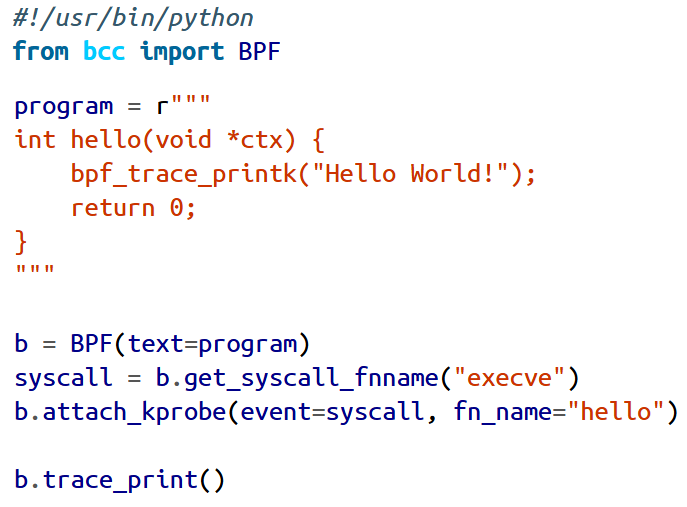
\includegraphics[scale=0.5]{ebpfProgramExample.png} % 在导演去导入了图片以后,这里就不要再包含后缀名
        \caption{测试代码}
        \label{fig3}
    \end{figure}

    所用表格为表 \ref{tbl1} 和表 \ref{tbl2}。
    \begin{table*}[htp]
        \centering
        \caption{数学字体对照表}
        \begin{threeparttable}
        % resizebox 使表格适应文档的宽度。
        % \resizebox{\columnwidth}{!}{  
        \xiaowu
        \begin{tabular}{*{18}{l}}
            \toprule
            \multicolumn{2}{c}{\texttt{mathrm}} & \multicolumn{2}{c}{\texttt{mathbf}} & \multicolumn{2}{c}{\texttt{mathit}} & \multicolumn{2}{c}{\texttt{mathsf}} & \multicolumn{2}{c}{\texttt{mathtt}} & \multicolumn{2}{c}{\texttt{mathcal}} & \multicolumn{2}{c}{\texttt{mathbb}} & \multicolumn{2}{c}{\texttt{mathfrak}} & \multicolumn{2}{c}{\texttt{mathscr}} \\ 
            \midrule
            $\mathrm{Aa}$ & $\mathrm{Nn}$ & $\mathbf{Aa}$ & $\mathbf{Nn}$ & $\mathit{Aa}$ & $\mathit{Nn}$ & $\mathsf{Aa}$ & $\mathsf{Nn}$ & $\mathtt{Aa}$ & $\mathtt{Nn}$ & $\mathcal{Aa}$ & $\mathcal{Nn}$ & $\mathbb{A}$ & $\mathbb{N}$ & $\mathfrak{Aa}$ & $\mathfrak{Nn}$ & $\mathscr{Aa}$ & $\mathscr{Nn}$ \\
            $\mathrm{Bb}$ & $\mathrm{Oo}$ & $\mathbf{Bb}$ & $\mathbf{Oo}$ & $\mathit{Bb}$ & $\mathit{Oo}$ & $\mathsf{Bb}$ & $\mathsf{Oo}$ & $\mathtt{Bb}$ & $\mathtt{Oo}$ & $\mathcal{Bb}$ & $\mathcal{Oo}$ & $\mathbb{B}$ & $\mathbb{O}$ & $\mathfrak{Bb}$ & $\mathfrak{Oo}$ & $\mathscr{Bb}$ & $\mathscr{Oo}$ \\
            $\mathrm{Cc}$ & $\mathrm{Pp}$ & $\mathbf{Cc}$ & $\mathbf{Pp}$ & $\mathit{Cc}$ & $\mathit{Pp}$ & $\mathsf{Cc}$ & $\mathsf{Pp}$ & $\mathtt{Cc}$ & $\mathtt{Pp}$ & $\mathcal{Cc}$ & $\mathcal{Pp}$ & $\mathbb{C}$ & $\mathbb{P}$ & $\mathfrak{Cc}$ & $\mathfrak{Pp}$ & $\mathscr{Cc}$ & $\mathscr{Pp}$ \\
            $\mathrm{Dd}$ & $\mathrm{Qq}$ & $\mathbf{Dd}$ & $\mathbf{Qq}$ & $\mathit{Dd}$ & $\mathit{Qq}$ & $\mathsf{Dd}$ & $\mathsf{Qq}$ & $\mathtt{Dd}$ & $\mathtt{Qq}$ & $\mathcal{Dd}$ & $\mathcal{Qq}$ & $\mathbb{D}$ & $\mathbb{Q}$ & $\mathfrak{Dd}$ & $\mathfrak{Qq}$ & $\mathscr{Dd}$ & $\mathscr{Qq}$ \\
            $\mathrm{Ee}$ & $\mathrm{Rr}$ & $\mathbf{Ee}$ & $\mathbf{Rr}$ & $\mathit{Ee}$ & $\mathit{Rr}$ & $\mathsf{Ee}$ & $\mathsf{Rr}$ & $\mathtt{Ee}$ & $\mathtt{Rr}$ & $\mathcal{Ee}$ & $\mathcal{Rr}$ & $\mathbb{E}$ & $\mathbb{R}$ & $\mathfrak{Ee}$ & $\mathfrak{Rr}$ & $\mathscr{Ee}$ & $\mathscr{Rr}$ \\
            $\mathrm{Ff}$ & $\mathrm{Ss}$ & $\mathbf{Ff}$ & $\mathbf{Ss}$ & $\mathit{Ff}$ & $\mathit{Ss}$ & $\mathsf{Ff}$ & $\mathsf{Ss}$ & $\mathtt{Ff}$ & $\mathtt{Ss}$ & $\mathcal{Ff}$ & $\mathcal{Ss}$ & $\mathbb{F}$ & $\mathbb{S}$ & $\mathfrak{Ff}$ & $\mathfrak{Ss}$ & $\mathscr{Ff}$ & $\mathscr{Ss}$ \\
            $\mathrm{Gg}$ & $\mathrm{Tt}$ & $\mathbf{Gg}$ & $\mathbf{Tt}$ & $\mathit{Gg}$ & $\mathit{Tt}$ & $\mathsf{Gg}$ & $\mathsf{Tt}$ & $\mathtt{Gg}$ & $\mathtt{Tt}$ & $\mathcal{Gg}$ & $\mathcal{Tt}$ & $\mathbb{G}$ & $\mathbb{T}$ & $\mathfrak{Gg}$ & $\mathfrak{Tt}$ & $\mathscr{Gg}$ & $\mathscr{Tt}$ \\
            $\mathrm{Hh}$ & $\mathrm{Uu}$ & $\mathbf{Hh}$ & $\mathbf{Uu}$ & $\mathit{Hh}$ & $\mathit{Uu}$ & $\mathsf{Hh}$ & $\mathsf{Uu}$ & $\mathtt{Hh}$ & $\mathtt{Uu}$ & $\mathcal{Hh}$ & $\mathcal{Uu}$ & $\mathbb{H}$ & $\mathbb{U}$ & $\mathfrak{Hh}$ & $\mathfrak{Uu}$ & $\mathscr{Hh}$ & $\mathscr{Uu}$ \\
            $\mathrm{Ii}$ & $\mathrm{Vv}$ & $\mathbf{Ii}$ & $\mathbf{Vv}$ & $\mathit{Ii}$ & $\mathit{Vv}$ & $\mathsf{Ii}$ & $\mathsf{Vv}$ & $\mathtt{Ii}$ & $\mathtt{Vv}$ & $\mathcal{Ii}$ & $\mathcal{Vv}$ & $\mathbb{I}$ & $\mathbb{V}$ & $\mathfrak{Ii}$ & $\mathfrak{Vv}$ & $\mathscr{Ii}$ & $\mathscr{Vv}$ \\
            $\mathrm{Jj}$ & $\mathrm{Ww}$ & $\mathbf{Jj}$ & $\mathbf{Ww}$ & $\mathit{Jj}$ & $\mathit{Ww}$ & $\mathsf{Jj}$ & $\mathsf{Ww}$ & $\mathtt{Jj}$ & $\mathtt{Ww}$ & $\mathcal{Jj}$ & $\mathcal{Ww}$ & $\mathbb{J}$ & $\mathbb{W}$ & $\mathfrak{Jj}$ & $\mathfrak{Ww}$ & $\mathscr{Jj}$ & $\mathscr{Ww}$ \\
            $\mathrm{Kk}$ & $\mathrm{Xx}$ & $\mathbf{Kk}$ & $\mathbf{Xx}$ & $\mathit{Kk}$ & $\mathit{Xx}$ & $\mathsf{Kk}$ & $\mathsf{Xx}$ & $\mathtt{Kk}$ & $\mathtt{Xx}$ & $\mathcal{Kk}$ & $\mathcal{Xx}$ & $\mathbb{K}$ & $\mathbb{X}$ & $\mathfrak{Kk}$ & $\mathfrak{Xx}$ & $\mathscr{Kk}$ & $\mathscr{Xx}$ \\
            $\mathrm{Ll}$ & $\mathrm{Yy}$ & $\mathbf{Ll}$ & $\mathbf{Yy}$ & $\mathit{Ll}$ & $\mathit{Yy}$ & $\mathsf{Ll}$ & $\mathsf{Yy}$ & $\mathtt{Ll}$ & $\mathtt{Yy}$ & $\mathcal{Ll}$ & $\mathcal{Yy}$ & $\mathbb{L}$ & $\mathbb{Y}$ & $\mathfrak{Ll}$ & $\mathfrak{Yy}$ & $\mathscr{Ll}$ & $\mathscr{Yy}$ \\
            $\mathrm{Mm}$ & $\mathrm{Zz}$ & $\mathbf{Mm}$ & $\mathbf{Zz}$ & $\mathit{Mm}$ & $\mathit{Zz}$ & $\mathsf{Mm}$ & $\mathsf{Zz}$ & $\mathtt{Mm}$ & $\mathtt{Zz}$ & $\mathcal{Mm}$ & $\mathcal{Zz}$ & $\mathbb{M}$ & $\mathbb{Z}$ & $\mathfrak{Mm}$ & $\mathfrak{Zz}$ & $\mathscr{Mm}$ & $\mathscr{Zz}$ \\
            \bottomrule
        \end{tabular}
        % }
        \begin{tablenotes}
            \item \xiaowu\songti{注:此数据仅为示例,实际数据可能有所不同.}
        \end{tablenotes}
        \end{threeparttable}
        \label{tbl1}
    \end{table*}
    \clearpage
    % https://tex.stackexchange.com/a/722703
    \begin{table}[ht]
        \centering
        \caption{各组分$\lg(B_i)$值}
        \wuhao
        \begin{threeparttable}
            \begin{tblr}{
                row{1} = {c},
                column{1} = {c},
                cell{1}{2} = {c=2}{},
                cell{1}{4} = {c=2}{},
                hline{1,3,18} = {-}{0.08em},
                hline{2} = {2-5}{0.08em},
            }
                \song{序号} & T=1500K &             & T=2000K    &           \\
                & \song{组分}      & $\lg(B_i)$  & \song{组分}& $\lg(B_i)$ \\
                1  & \ce{O2+}        & 5.26         & \ce{HO2}  & 6.43     \\
                2  & \ce{HO2}        & 5.26         & \ce{O2+}  & 6.42     \\
                3  & \ce{H2O+}       & 4.76         & \ce{H2O+} & 6.18     \\
                4  & \ce{N2+}        & 3.97         & \ce{H}    & 6.12     \\
                5  & \ce{H}          & 3.54         & \ce{H2+}  & 6.04     \\
                6  & \ce{OH}         & 3.29         & \ce{OH}   & 5.91     \\
                7  & \ce{CO+}        & 3.26         & \ce{O}    & 5.59     \\
                8  & \ce{H2+}        & 2.54         & \ce{N2+}  & 4.87     \\
                9  & \ce{O}          & 2.30         & \ce{CO+}  & 3.98     \\
                10 & \ce{H2O2}       & 1.62         & \ce{CO2+} & 3.76     \\
                11 & \ce{CO2+}       & 1.40         & \ce{H2O2} & 3.09     \\
                12 & \ce{HCO}\tnote{*}& -0.47       & \ce{HCO}\tnote{*}& 0.24     \\
                13 & \ce{N+}         & -4.85        & \ce{N+}   & -2.81    \\
                14 & \ce{CH2O+}      & -6.91        & \ce{CH2O}\tnote{*}& -6.13    \\
                15 & \ce{NO+}        & -16.60       & \ce{NO+}  & -11.76     
            \end{tblr}
            \obeylines\medskip
            \xiaowu\songti{注:“+”表示重要组分,“*”表示冗余组分.}
            % \obeylines
            % \xiaowu\songti{注:“+”表示重要组分,“\item[*]”表示冗余组分.} wrap 在 footnote 里。
        \end{threeparttable}
        \label{tbl2}
    \end{table}}
        \xiaosi{% 没有附录的,就不include/input进来。
\addcontentsline{toc}{section}{附录}
\setAppendixHere{A}
    % 需要用 \eqref 才会加圆括号。
    公式如 \eqref{eq1} 式所示。所形成的交换图如图 \ref{fig1},图 \ref{fig2},图 \ref{fig3} 和图 \ref{performanceOfSCLL} 所示。
    \begin{equation}
        \begin{aligned}
            \int \frac{x+\sin x}{1 + \cos x} \mathrm{d} x &= \int \frac{x}{2\cos^2 \frac{x}{2}} + \tan \frac{x}{2} \mathrm{d} x \\
                &= \int x\mathrm{d}\tan \frac{x}{2} + \tan \frac{x}{2} \mathrm{d} x \\
                &= \frac{x}{2}\tan \frac{x}{2} - \int \tan \frac{x}{2} \mathrm{d} x + \int \tan \frac{x}{2} \mathrm{d} x \\
                &= x\tan \frac{x}{2} + C 
        \end{aligned}
        \label{eq1}
    \end{equation}
    \begin{figure*}[htb]
        \centering
        \begin{tikzcd}
            A \arrow[r, "\phi"] \arrow[d, red]
            & B \arrow[d, "\psi" red] \\
            C \arrow[r, red, "\eta" blue]
            & |[blue, rotate=-15]| D
        \end{tikzcd}
        % 注意标签一定要放在提供给 ref 的 label 之前否则会出现??.
        \caption{{交换图例一}}
        \label{fig1}
    \end{figure*}
    \begin{figure*}[htb]
        \centering
        \begin{tikzcd}[column sep=tiny]
            & \pi_1(U_1) \ar[dr]\ar[drr, "j_1", bend left=20] &&[1.5em] \\
            \pi_1(U_1\cap U_2) \ar[ur,"i_1"] \ar[dr, "i_2"swap] && \pi_1(U_1) \ast_{\pi_1(U_1\cap U_2)}
            \pi_1(U_2) \ar[r, dashed, "\simeq"] & \pi_1(X) \\
            & \pi_1(U_2) \ar[ur]\ar[urr, "j_2"swap, bend right=20]
            &&
        \end{tikzcd}
        % 手工插入间距
        \vspace{0.5em}\par{\xiaowu{注:关系与图\ref{fig1}类似,但不多.}}
        \caption{{交换图例二}}
        \label{fig2}
    \end{figure*}
    \begin{figure*}[htb]
        \centering
        \begin{tikzcd}
            T
            \arrow[drr, bend left, "x"]
            \arrow[ddr, bend right, "y"]
            \arrow[dr, dotted,background color=blue!20,
            "{(x,y)}"description] & & \\
            & X \times_Z Y \arrow[r, "p"] \arrow[d, "q"]
            & X \arrow[d, "f"] \\
            & Y \arrow[r, "g"]
            & Z
        \end{tikzcd}
        % 手工插入间距
        \vspace{0.5em}\par{\xiaowu{注:关系与图\ref{fig1},图\ref{fig2}类似,但不多.}}
        \caption{{交换图例三}}
        \label{fig3}
    \end{figure*}
    \begin{figure}[htb]
        \centering
        % TimeResults
        \begin{tikzpicture}
            \begin{axis}[
                ylabel={用时(s)},
                xlabel={执行轮数},
                legend columns=7,
                legend style={at={(1.5,-0.3)},anchor=outer south},
                % 如果有多个子图,可以用groupplot来。
                % 具体不教,自己看手册去。
                % title={},
                yticklabel style={
                    /pgf/number format/.cd, 
                    /pgf/number format/fixed,
                    /pgf/number format/precision=3
                }
            ]
            \addplot [
                scatter,
                only marks,
                point meta=explicit symbolic,
                scatter/classes={
                    correlation={mark=square*,blue},
                    covariance={mark=triangle*,red},
                    gemm={mark=o,draw=black},
                    gemver={mark=x,draw=green},
                    ludcmp={mark=o,draw=cyan},
                    nussinov={mark=x,draw=blue},
                    seidel-2d={mark=triangle*,yellow}% <-- don't add comma
                },
            ] table [meta=label] {\TimeResults};
            \legend{correlation,covariance,gemm, gemver, ludcmp, nussinov, seidel-2d};
            \end{axis} 
        \end{tikzpicture} 
        \caption{性能统计图表}
        \label{performanceOfSCLL}
    \end{figure}
    \newpage

\setAppendixHere{B}
    \begin{figure}[htb]
        \centering
        \subcaptionbox{湖南}{
\includegraphics[width=.24\linewidth]{HSVGPDF.jpg}}
        \subcaptionbox{大学}{
\includegraphics[width=.24\linewidth]{HSVGPDF-transparent.png}}
        \caption{所用代码集}
        \label{fig4}
    \end{figure}

    所用图片为图 \ref{fig4}。所用表格为表 \ref{tbl1} 和表 \ref{tbl2}。

    {\wuhao{
        \setlength\tabcolsep{2pt}
        \begin{longtable}{*{18}{l}}
            \caption{数学字体对照表}
            \label{tbl1}\\
            \specialrule{1pt}{0pt}{0pt}
            \multicolumn{2}{c}{\texttt{mathrm}} & \multicolumn{2}{c}{\texttt{mathbf}} & \multicolumn{2}{c}{\texttt{mathit}} & \multicolumn{2}{c}{\texttt{mathsf}} & \multicolumn{2}{c}{\texttt{mathtt}} & \multicolumn{2}{c}{\texttt{mathcal}} & \multicolumn{2}{c}{\texttt{mathbb}} & \multicolumn{2}{c}{\texttt{mathfrak}} & \multicolumn{2}{c}{\texttt{mathscr}} \\ 
            \hline
            \endfirsthead
            \multicolumn{18}{l}{(续上页表\ref{tbl1})}\\
            \specialrule{1pt}{0pt}{0pt}
            \multicolumn{2}{c}{\texttt{mathrm}} & \multicolumn{2}{c}{\texttt{mathbf}} & \multicolumn{2}{c}{\texttt{mathit}} & \multicolumn{2}{c}{\texttt{mathsf}} & \multicolumn{2}{c}{\texttt{mathtt}} & \multicolumn{2}{c}{\texttt{mathcal}} & \multicolumn{2}{c}{\texttt{mathbb}} & \multicolumn{2}{c}{\texttt{mathfrak}} & \multicolumn{2}{c}{\texttt{mathscr}} \\ 
            \hline
            \endhead
            \specialrule{1pt}{0pt}{0pt}
            \multicolumn{11}{l}{\xiaowu{注:此数据仅为示例,实际数据可能有所不同.}}\\
            \endlastfoot
            \specialrule{1pt}{0pt}{0pt}
            \multicolumn{18}{r}{(表\ref{tbl1}接下页)}\\
            \endfoot
            $\mathrm{Aa}$ & $\mathrm{Nn}$ & $\mathbf{Aa}$ & $\mathbf{Nn}$ & $\mathit{Aa}$ & $\mathit{Nn}$ & $\mathsf{Aa}$ & $\mathsf{Nn}$ & $\mathtt{Aa}$ & $\mathtt{Nn}$ & $\mathcal{Aa}$ & $\mathcal{Nn}$ & $\mathbb{A}$ & $\mathbb{N}$ & $\mathfrak{Aa}$ & $\mathfrak{Nn}$ & $\mathscr{Aa}$ & $\mathscr{Nn}$ \\
            $\mathrm{Bb}$ & $\mathrm{Oo}$ & $\mathbf{Bb}$ & $\mathbf{Oo}$ & $\mathit{Bb}$ & $\mathit{Oo}$ & $\mathsf{Bb}$ & $\mathsf{Oo}$ & $\mathtt{Bb}$ & $\mathtt{Oo}$ & $\mathcal{Bb}$ & $\mathcal{Oo}$ & $\mathbb{B}$ & $\mathbb{O}$ & $\mathfrak{Bb}$ & $\mathfrak{Oo}$ & $\mathscr{Bb}$ & $\mathscr{Oo}$ \\
            $\mathrm{Cc}$ & $\mathrm{Pp}$ & $\mathbf{Cc}$ & $\mathbf{Pp}$ & $\mathit{Cc}$ & $\mathit{Pp}$ & $\mathsf{Cc}$ & $\mathsf{Pp}$ & $\mathtt{Cc}$ & $\mathtt{Pp}$ & $\mathcal{Cc}$ & $\mathcal{Pp}$ & $\mathbb{C}$ & $\mathbb{P}$ & $\mathfrak{Cc}$ & $\mathfrak{Pp}$ & $\mathscr{Cc}$ & $\mathscr{Pp}$ \\
            $\mathrm{Dd}$ & $\mathrm{Qq}$ & $\mathbf{Dd}$ & $\mathbf{Qq}$ & $\mathit{Dd}$ & $\mathit{Qq}$ & $\mathsf{Dd}$ & $\mathsf{Qq}$ & $\mathtt{Dd}$ & $\mathtt{Qq}$ & $\mathcal{Dd}$ & $\mathcal{Qq}$ & $\mathbb{D}$ & $\mathbb{Q}$ & $\mathfrak{Dd}$ & $\mathfrak{Qq}$ & $\mathscr{Dd}$ & $\mathscr{Qq}$ \\
            $\mathrm{Ee}$ & $\mathrm{Rr}$ & $\mathbf{Ee}$ & $\mathbf{Rr}$ & $\mathit{Ee}$ & $\mathit{Rr}$ & $\mathsf{Ee}$ & $\mathsf{Rr}$ & $\mathtt{Ee}$ & $\mathtt{Rr}$ & $\mathcal{Ee}$ & $\mathcal{Rr}$ & $\mathbb{E}$ & $\mathbb{R}$ & $\mathfrak{Ee}$ & $\mathfrak{Rr}$ & $\mathscr{Ee}$ & $\mathscr{Rr}$ \\
            $\mathrm{Ff}$ & $\mathrm{Ss}$ & $\mathbf{Ff}$ & $\mathbf{Ss}$ & $\mathit{Ff}$ & $\mathit{Ss}$ & $\mathsf{Ff}$ & $\mathsf{Ss}$ & $\mathtt{Ff}$ & $\mathtt{Ss}$ & $\mathcal{Ff}$ & $\mathcal{Ss}$ & $\mathbb{F}$ & $\mathbb{S}$ & $\mathfrak{Ff}$ & $\mathfrak{Ss}$ & $\mathscr{Ff}$ & $\mathscr{Ss}$ \\
            $\mathrm{Gg}$ & $\mathrm{Tt}$ & $\mathbf{Gg}$ & $\mathbf{Tt}$ & $\mathit{Gg}$ & $\mathit{Tt}$ & $\mathsf{Gg}$ & $\mathsf{Tt}$ & $\mathtt{Gg}$ & $\mathtt{Tt}$ & $\mathcal{Gg}$ & $\mathcal{Tt}$ & $\mathbb{G}$ & $\mathbb{T}$ & $\mathfrak{Gg}$ & $\mathfrak{Tt}$ & $\mathscr{Gg}$ & $\mathscr{Tt}$ \\
            $\mathrm{Hh}$ & $\mathrm{Uu}$ & $\mathbf{Hh}$ & $\mathbf{Uu}$ & $\mathit{Hh}$ & $\mathit{Uu}$ & $\mathsf{Hh}$ & $\mathsf{Uu}$ & $\mathtt{Hh}$ & $\mathtt{Uu}$ & $\mathcal{Hh}$ & $\mathcal{Uu}$ & $\mathbb{H}$ & $\mathbb{U}$ & $\mathfrak{Hh}$ & $\mathfrak{Uu}$ & $\mathscr{Hh}$ & $\mathscr{Uu}$ \\
            $\mathrm{Ii}$ & $\mathrm{Vv}$ & $\mathbf{Ii}$ & $\mathbf{Vv}$ & $\mathit{Ii}$ & $\mathit{Vv}$ & $\mathsf{Ii}$ & $\mathsf{Vv}$ & $\mathtt{Ii}$ & $\mathtt{Vv}$ & $\mathcal{Ii}$ & $\mathcal{Vv}$ & $\mathbb{I}$ & $\mathbb{V}$ & $\mathfrak{Ii}$ & $\mathfrak{Vv}$ & $\mathscr{Ii}$ & $\mathscr{Vv}$ \\
            $\mathrm{Jj}$ & $\mathrm{Ww}$ & $\mathbf{Jj}$ & $\mathbf{Ww}$ & $\mathit{Jj}$ & $\mathit{Ww}$ & $\mathsf{Jj}$ & $\mathsf{Ww}$ & $\mathtt{Jj}$ & $\mathtt{Ww}$ & $\mathcal{Jj}$ & $\mathcal{Ww}$ & $\mathbb{J}$ & $\mathbb{W}$ & $\mathfrak{Jj}$ & $\mathfrak{Ww}$ & $\mathscr{Jj}$ & $\mathscr{Ww}$ \\
            $\mathrm{Kk}$ & $\mathrm{Xx}$ & $\mathbf{Kk}$ & $\mathbf{Xx}$ & $\mathit{Kk}$ & $\mathit{Xx}$ & $\mathsf{Kk}$ & $\mathsf{Xx}$ & $\mathtt{Kk}$ & $\mathtt{Xx}$ & $\mathcal{Kk}$ & $\mathcal{Xx}$ & $\mathbb{K}$ & $\mathbb{X}$ & $\mathfrak{Kk}$ & $\mathfrak{Xx}$ & $\mathscr{Kk}$ & $\mathscr{Xx}$ \\
            $\mathrm{Ll}$ & $\mathrm{Yy}$ & $\mathbf{Ll}$ & $\mathbf{Yy}$ & $\mathit{Ll}$ & $\mathit{Yy}$ & $\mathsf{Ll}$ & $\mathsf{Yy}$ & $\mathtt{Ll}$ & $\mathtt{Yy}$ & $\mathcal{Ll}$ & $\mathcal{Yy}$ & $\mathbb{L}$ & $\mathbb{Y}$ & $\mathfrak{Ll}$ & $\mathfrak{Yy}$ & $\mathscr{Ll}$ & $\mathscr{Yy}$ \\
            $\mathrm{Mm}$ & $\mathrm{Zz}$ & $\mathbf{Mm}$ & $\mathbf{Zz}$ & $\mathit{Mm}$ & $\mathit{Zz}$ & $\mathsf{Mm}$ & $\mathsf{Zz}$ & $\mathtt{Mm}$ & $\mathtt{Zz}$ & $\mathcal{Mm}$ & $\mathcal{Zz}$ & $\mathbb{M}$ & $\mathbb{Z}$ & $\mathfrak{Mm}$ & $\mathfrak{Zz}$ & $\mathscr{Mm}$ & $\mathscr{Zz}$ \\    
        \end{longtable}
        \setlength\tabcolsep{1.5em}
        \begin{longtable}{c|c|c|c|c}
            \caption{方法 — 干扰抑制结果}
            \label{ref-longtable}\\
            \specialrule{1pt}{0pt}{0pt}
            干扰类型 &目标信号 &阵元数 &干扰采样值数 &SINR(dB)\\
            \hline
            \endfirsthead
            \specialrule{1pt}{0pt}{0pt}
            \endfoot
            \multirow{4}{*}{第一类干扰} &\multirow{2}{*}{信号1} &8 &—— &30.58\\
            \cline{3-5}
            &&4 &—— &21.16\\
            \cline{2-5}
            &\multirow{2}{*}{信号4}&8 &—— &38.28\\
            \cline{3-5}
            &&4 &—— &38.28\\
            \hline
            \multirow{3}{*}{第二类干扰} &\multirow{3}{*}{信号4} &\multirow{2}{*}{8} &30 &4.69\\
            \cline{4-5}
            &&&19 &4.83\\
            \cline{3-5}
            &&4 &30 &-0.42\\
        \end{longtable}
        \begin{longtable}{*{5}{c}} 
            \caption{各组分 $\lg(B_i)$ 值}
            \label{tbl2}\\
            \specialrule{1pt}{0pt}{0pt}
            序号 & \multicolumn{2}{c}{T=1500K} & \multicolumn{2}{c}{T=2000K}  \\ 
            \cline{2-5}
            & 组分                   & $\lg B_i$   & 组分                  & $\lg B_i$ \\ 
            \hline
            \endfirsthead

            \multicolumn{5}{l}{(接上页表\ref{tbl2})} \\
            \specialrule{1pt}{0pt}{0pt}
            序号 & \multicolumn{2}{c}{T=1500K} & \multicolumn{2}{c}{T=2000K}  \\ 
            \cline{2-5}
            & 组分                   & $\lg B_i$   & 组分                  & $\lg B_i$ \\ 
            \hline
            \endhead

            \specialrule{1pt}{0pt}{0pt}
            \multicolumn{5}{l}{\xiaowu{注:“+”表示重要成分,“*”表示冗余组分.}} \\
            \endlastfoot

            \specialrule{1pt}{0pt}{0pt}
            \multicolumn{5}{r}{(表\ref{tbl2}接下页)} \\
            \endfoot

            1  & \ce{O2}\TblrNote{+}   &   5.26      & \ce{HO2}              &  6.43    \\
            2  & \ce{HO2}              &   5.26      & \ce{O2}\TblrNote{+}   &  6.42    \\
            3  & \ce{H2O}\TblrNote{+}  &   4.76      & \ce{H2O}\TblrNote{+}  &  6.18    \\
            4  & \ce{N2}\TblrNote{+}   &   3.97      & \ce{H}                &  6.12    \\
            5  & \ce{H}                &   3.54      & \ce{H2}\TblrNote{+}   &  6.04    \\
            6  & \ce{OH}               &   3.29      & \ce{OH}               &  5.91    \\
            7  & \ce{CO}\TblrNote{+}   &   3.26      & \ce{O}                &  5.59    \\
            8  & \ce{H2}\TblrNote{+}   &   2.54      & \ce{N2}\TblrNote{+}   &  4.87    \\
            9  & \ce{O}                &   2.30      & \ce{CO}\TblrNote{+}   &  3.98    \\
            10 & \ce{H2O2}             &   1.62      & \ce{CO2}\TblrNote{+}  &  3.76    \\
            11 & \ce{CO2}\TblrNote{+}  &   1.40      & \ce{H2O2}             &  3.09    \\
            12 & \ce{HCO}\TblrNote{*}  &   -0.47     & \ce{HCO}\TblrNote{*}  &  0.24    \\
            13 & \ce{N}\TblrNote{+}    &   -4.85     & \ce{N}\TblrNote{+}    &  -2.81   \\
            14 & \ce{CH2O}\TblrNote{+} &   -6.91     & \ce{CH2O}\TblrNote{*} &  -6.13   \\
            15 & \ce{NO}\TblrNote{+}   &   -16.60    & \ce{NO}\TblrNote{+}   &  -11.76  \\                    
        \end{longtable}
        \begin{longtable}{@{}m{4em}<{\centering}|m{7em}<{\centering}|m{8em}<{\centering}|c<{\centering}|m{4em}<{\centering}@{}}
            \caption{电子文献标识类型}
            \label{OL-types}\\
            \specialrule{1pt}{0pt}{0pt}
            类型 &数据库(网上) &计算机程序(磁盘) &电子公告(网上) &光盘图书\\
            \hline
            \endfirsthead
            \specialrule{1pt}{0pt}{0pt}
            \endfoot
            文献标识符 &DB(DB/OL) &CP(CP/DK) &EB(EB/OL) &M/CD\\
        \end{longtable}
        \begin{longtable}{c|c|c|c|c|c}
            \caption{参考文献标识类型}
            \label{ref-types}\\
            \specialrule{1pt}{0pt}{0pt}
            类型 &专著 &会议录 &(单篇论文) &报纸文章 &期刊文章\\
            \hline
            \endfirsthead
            \specialrule{1pt}{0pt}{0pt}
            \endfoot
            文献标识符 &M &C &A &N &J\\
            \hline
            类型 &学位论文 &报告 &标准 &专利 &其它文献\\
            \hline
            文献标识符 &D &R &S &P &Z\\
        \end{longtable}
    }}

\setAppendixHere{C}
    \vspace{-4em}
    {
        \wuhao{\printunsrtglossary[style=CustomSymbolTableStyle, title={}]}
    }}
    \end{sloppypar}
\end{document}
